\documentclass[main.tex]{subfiles}

\begin{document}

\chapter{Testing \& Evaluation}

\section{Step Dectection}

Step detection is an integral part of any dead-reckoning system and as such, 
it is prudent to test this particular component in isolation to try and ascertain how much error within the whole system is attributable to the step detection.
As mentioned previously, different methods were implemented to try and find the best step detection system, resulting in three step detection algorithm implmentations that needed testing:
\begin{enumerate}
	\item First Order Low Pass Filter
	\item 10th Order Butterworth Filter
	\item 5th Order Butterworth Filter
\end{enumerate}

Originally, the Basic Peak-Valley detection was also considered for testing as it forms the basis of how steps are detected in all future methods, making it a useful baseline comparison for all results. However, if it is completely unfiltered, then it will simply accept most actions as a step, whilst if it is flitered, then often no action will trigger a step. As such, it is not suited for analysis as a standalone entity, forcing us to forgo these plans.

All tests are done on a device of each operating system (Android/iOS) with six different users. This should allow for these tests to prove that the application works independently of user and device.

\subsection{Error Rate}

The error rate for the Step Detection algorithms is defined as follows:

\begin{equation}
Error\ Rate = 1 - \frac{Counted\ Value}{True\ Value}
\end{equation}

Over a given walk, the number of steps counted by the algorithm is divided by the true value of steps taken to determine the proportion of steps detected. Subtracting this value from 1 gives an overall error rate, with values close to 0 indicating favourable error rates.

%So over a known number of steps, True Value, each algorithm is used and its counted number of steps is used to get it's accuracy. From this is then subtracted from 1 to get the error rate. The purpose is to see over a set distance how much error is present overall regardless of timing or other factors such as speed, location etc... This should help to see how much where in the future the system can be improved.


\begin{table}[ht]
	\begin{tabular}{| c || c | c | c | c | c | c | c | c | c | c | c | c |}
		\hline
		True & \multicolumn{4}{c}{Low Pass} & \multicolumn{4}{|c|}{5th Butterworth} & \multicolumn{4}{c|}{10th Butterworth} \\
		\hline
		 - & Andr. & Err. & iOS & Err. & Andr. & Err. & iOS & Err. & Andr. & Err. & iOS & Err.\\
		\hline
		10 & 9.3 & 0.07 & 9.33 & 0.07 & 10 & 0.0 & 10 & 0.0 & 10 & 0.0 & 10 & 0.0 \\ 		
		25 & 22.8 & 0.09 & 22.5 & 0.1 & 24.5 & 0.02 & 24 & 0.04 & 26 & -0.04 & 25.7 & -0.03 \\ 	
		50 & 46.5 & 0.07 & 47.33 & 0.05 & 48.3 & 0.03 & 47.8 & 0.04 & 51.3 & -0.03 & 47 & 0.06\\ 
		\hline	
	\end{tabular}
	\caption{The average data recorded from all users.}
\end{table}

The above table shows the number of steps the each step detector counter against the true value. Three different true values where selected to see whether distance would have an impact on error build up. The highest true value, 50, was selected because this is roughly at most the number of steps a user will take to navigate within the environment. 

From the table above it can be see that the error remains fairly consistent across the different steps taken. This is somewhat expected, given the accelerometer is not subject to the drift that the gyroscope suffers from. For 10 steps, all algorithms show almost perfect results. As steps increase, it can be clearly seen that both implementations of the butterworth filter are superior to the low pass filter, with the low pass filter showing the largest error rates within both the 25 and 50 steps tests.

Selecting between the 5th and 10th order butterworth filters is more difficult when accounting for error rates alone, since both show similar results, although the 5th order filter is slightly superior. What works against the 10th order filter is the larger 'lag' registered with it  , with the time between taking a step and the step being recorded being greater for the 10th order filter. This is shown in figure ~\ref{fig:pirate}. Given all this, as has been mentioned previously, the 5th order Butterworth filter was selected as the step detection algorithm of choice, and it is the algorithm that was used for all other tests of the application.

\begin{center}
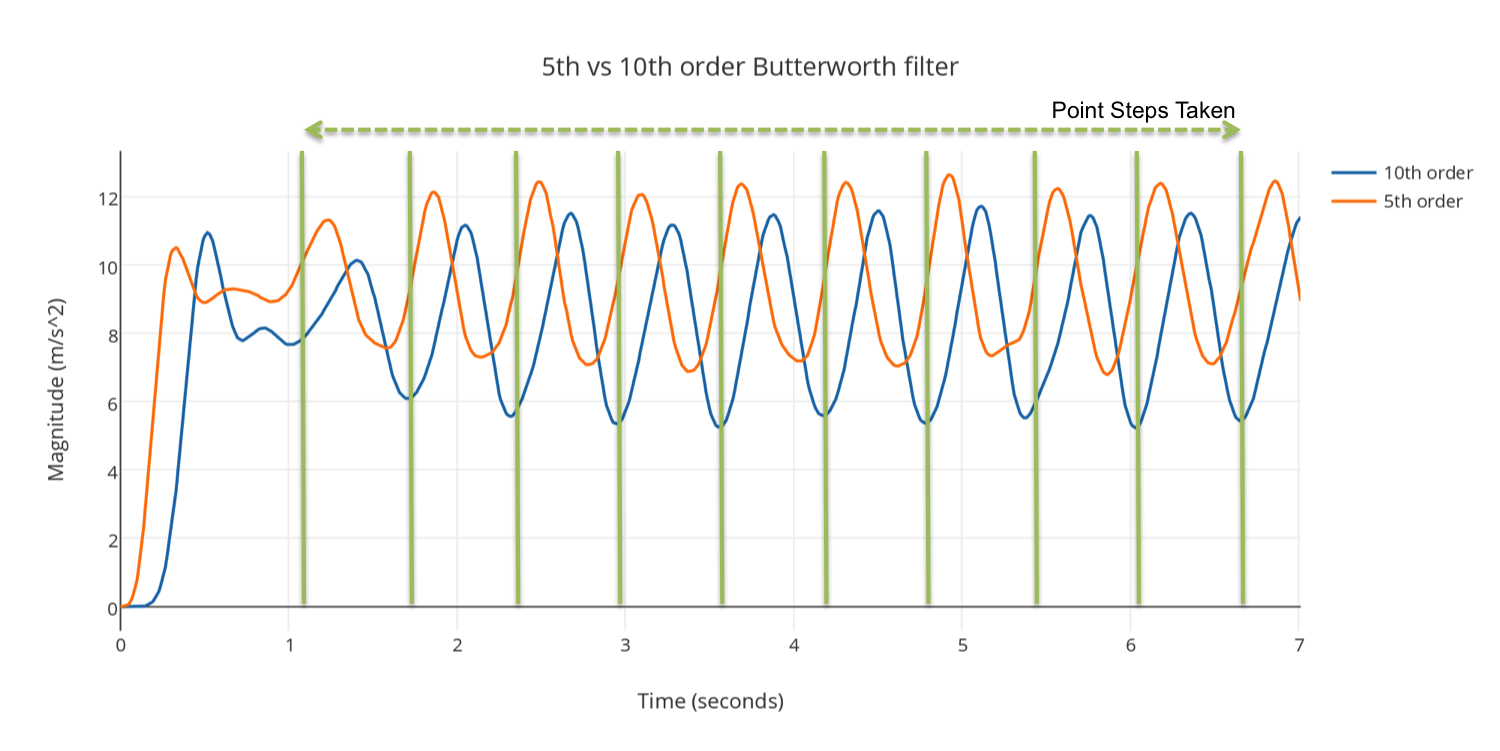
\includegraphics[scale=0.63]{images/pirateResults.png}
\captionof{figure}{Showing steps taken vs when acceleration peak occurs within 5th and 10th order Butterworth filters.}
\label{fig:pirate}
\end{center}

In this particular case, we considered that the underestimation and overestimation of steps are both equally detrimental, since both would result in the addition of an equal amount of error to the system.

%Though overcounting and getting a negative error rate could be considered worse than undercounting. This is because if you overcount it means that for a single step you will have counted an additional step, and in a dead-reckoning system the user will now have moved double the distance in a given direction by your estimate. This could have a larger effect on the error in the system.

\subsection{Proximity to Destination}

Having established that the 5th order Butterworth filter was the most appropriate algorithm for use, we proceeded to test the full application. It was tested along a series of routes that fell into two different categories:

\begin{enumerate}
	\item Room-to-Room, so from the entrance of one room to another  %, on the same floor
	\item Point-to-Point, from a specific starting location to a specific destination  %, on the same floor
%	\item Room to Room, across multiple floors
%	\item Point to Point across multiple floors
\end{enumerate}

We again had six different users walking along these routes. Upon the application stating that the destination had been reached, the distance between the users location and the actual location of the destination was measured in metres.

The purpose of this final test was to examine how well the application worked as a whole. The closer the proximity between the user's final location and the desired location, the more accurate the system can be deemed to be.

\begin{table}[ht]
	\begin{tabular}{| c || c | c | c | c |}
		\hline
		Route Number & Starting Location & Ending Location & Route Type & Proximity (m) \\
		\hline
		1 & CS0.06 & CS0.02 & RTR & 1.1 \\
		2 & CS0.03 (Top Right) & CS0.02 (Middle) & PTP & 3.4 (7.0) \\
		3 & CS0.07 & CS0.01 & RTR & 1.4 \\
		4 & CS0.06 (Bottom Left) & CS0.01 (Top Right) & PTP & 2.5\\ 
		5 & Entrance & Stairs & RTR & 1.7 \\
		5 & Stairs & CS1.16 & RTR & 2.6 (5.4) \\
		\hline
	\end{tabular}
	\label{tab:routes}
	\caption{The average proximity to destination, PTP means Point-to-Point, RTR means Room-to-Room}
\end{table}
%Results

Table ~\ref{tab:routes} shows the average distance to the destination for all users across the described routes (with each route being walked three times by each user). Some of the routes are shown in Figure [X]. The description in brackets for the PTP routes is the rough area of the room that the starting or ending location was placed. 5 routes in total were used, with the duplication of the route number 5 indicating a multi-floor route.

As can be seen, the overall error of the navigation for these routes ranged between 1m and 3.5m. In most cases, despite this error, navigation took the user within visual range of the desired destination, meaning that in a real world situation navigation would in most cases have been successful.

Two of the routes within the table have additional proximity values given within brackets. These are the rough distance away from the destination where the application stopped being able to track the user.  These instances occured when the system incorrectly believed the user to be facing a wall, cause all subsequent steps to trigger the wall collision mechanism and effectively cause the user to stop being tracked. This resulted from incorrect compass headings being recorded. We found that in certain locations around the computer science department building, specific areas of magnetic interference caused compass readings to fluctuate and become incorrect. These areas are shown in Figure ~\ref{fig:figureX}.

\begin{center}
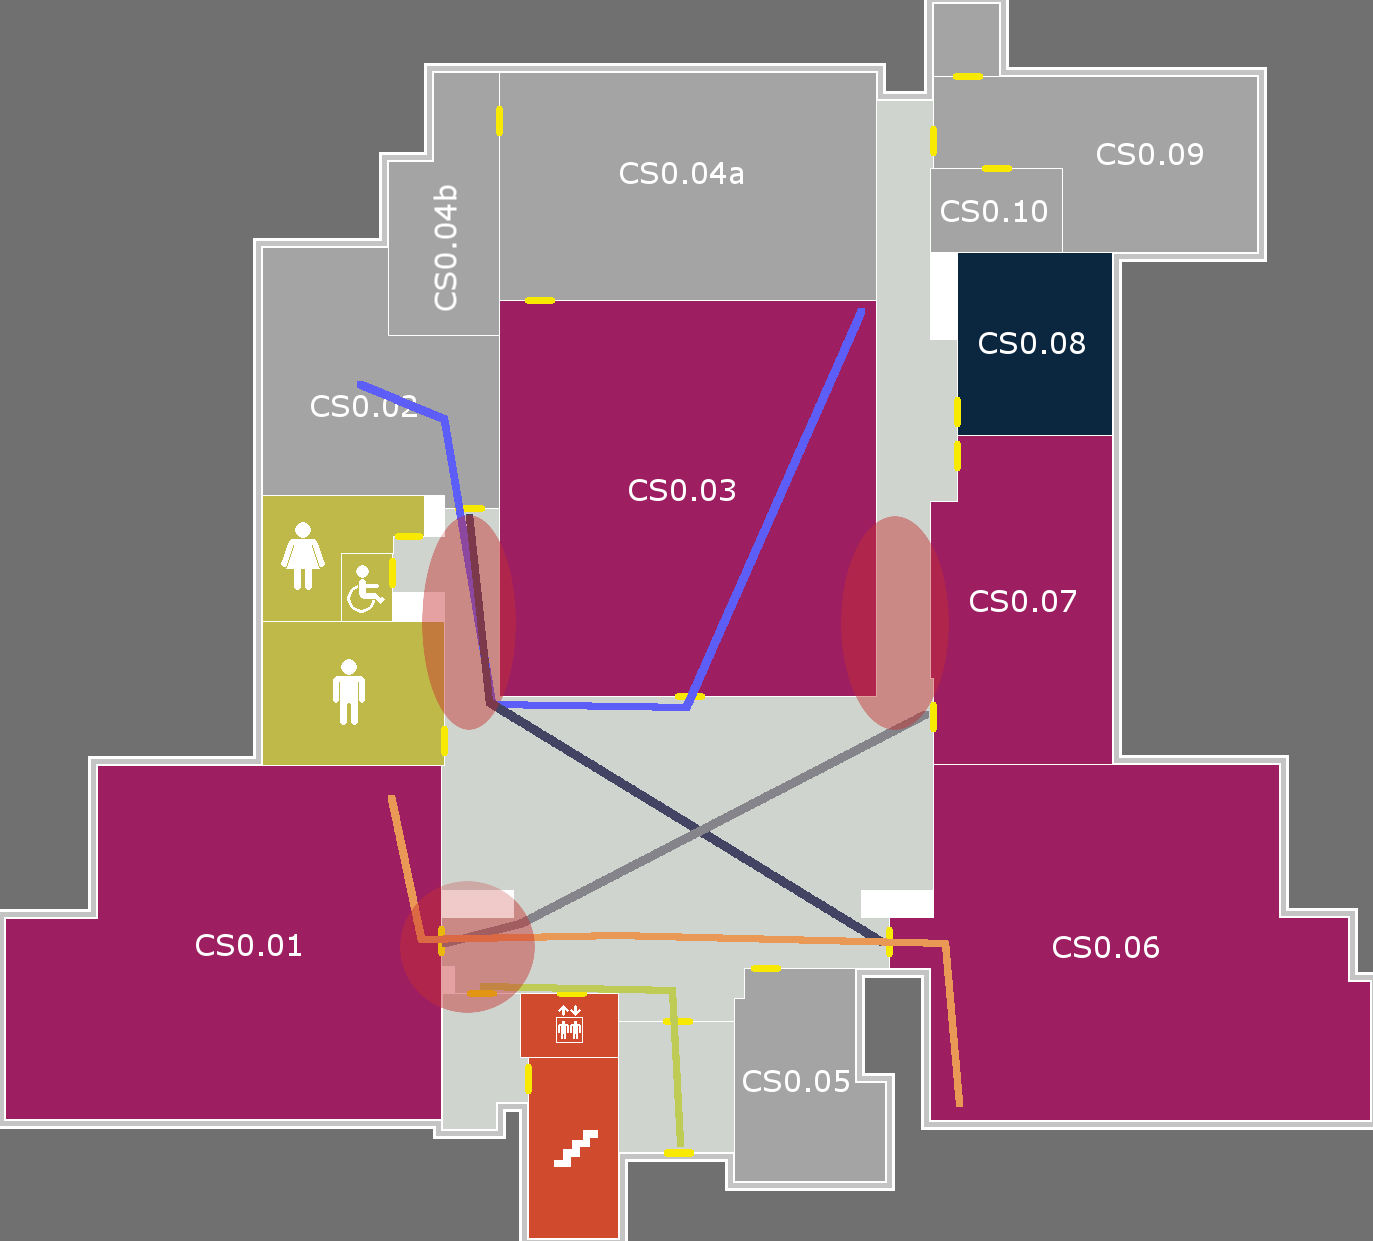
\includegraphics[scale=0.3]{images/figureX.png}
\captionof{figure}{Shows routes taken during testing. Red circles indicate encountered areas of magnetic interference with the compass.}
\label{fig:figureX}
\end{center}

These areas mean that dependening on the route taken by the user, it is possible for the error to cause significant problems. In cases where turns are made around narrow corners or small doorways are present in regions of magnetic interference, such as in route 2, these heading fluctuations cause the wall collision to be triggered and for tracking to fail. In route 1, where no such conditions exist, this problem does not occur. This phenomenon is shown within Figure ~\ref{fig:figureY}.

\begin{center}
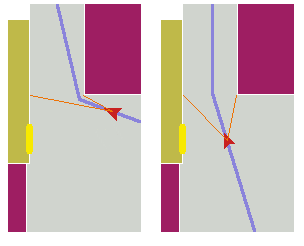
\includegraphics[scale=0.8]{images/figureY.png}
\captionof{figure}{The left side of the image demonstrates  that a sharper turn has a smaller range of heading error that will allow it to navigate the turn effectively. The image on the right demonstrates how reducing the steepness of the turn increases this range of error permitted for the turn to still take place.}
\label{fig:figureY}
\end{center}

Since our environment has several of these large pockets of interference, the application was tested in the concourse of the University Physics building, a location with less electronic equipment, the map of which is shown in Figure [Z]. The testing in this environment was to simply walk around, from a start point, with the phone facing a particular direction and see how the heading changed and the application tracked our location.

\begin{center}
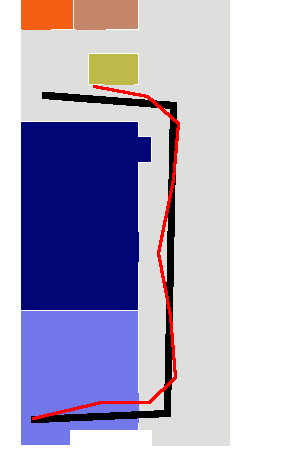
\includegraphics[scale=1]{images/figureZ.png}
\captionof{figure}{Floor plan of science concourse used to perform further tests on the compass.}
\label{fig:figureZ}
\end{center}

Despite having less electronic equipment in the area, we still noticed areas in which the compass value would incorrectly vary by as much as 20 degrees. Therefore, we can assume this interference is an artifact of the architecture and electricy used within the university's buildings. Overall this was an unexpected find. Early testing had failed to indicate such issues with the use of the compass, and from a theoretical perspective, we believed that any magnetic interefere would manifest in a more general offset rather than within small regions giving large spikes in readings.

With consistent compass readings, the system is however shown to be relatively accurate, wtll all completed navigation directing users to within visual contact of their targeted destinations.

\subsection{Other Considered Tests}

Two other tests where considered for use, but ultimately decided against for different reasons. The first was trying to measure if each step detector method was overcounting, registering multiple steps instead when it should only register a single. This is different from what was defined as a false positive earlier where a step is counted when no movement is occuring. This was considered as an alternative to the false positive rate as it looks at the way in which a bad algorithm could have a low error rate but not count correctly. 

However whilst this method could provide some analysis, it was not used for two reasons:

\begin{enumerate}
	\item All the methods being tested do not overcount often, it only really differentiates them from the basic unfiltered version.
	\item The second test that was not used would be better at showing which algorithms are working correctly
\end{enumerate}

The second test that was excluded was aiming to see if step detectors worked effectively over a period of time. The experiment was based off the fact that a person moving at a constant speed will have a repetitive waveform as the input into the algorithms. Therefore the steps being detected should be picked up constantly and equally spaced in time. The purpose of this test is to therefore show that an algorithm is matching the constant pattern and working as intended, it will show up any method that has a low error rate but doesn't work as intended. This was considered a better way to show what the overcounting test would have provided.

Whilst the method had some potential, early data recordings showed that all of the algorithms being tested had roughly the same pattern. They had the same pattern due to the need to have the timing relative to when it itself recorded the first step. Even though some methods recorded steps comparatively longer after they were actually taken, the timing results did not reflect that since the relative difference between when the steps as recorded by the algorithms themselves was similar


\end{document}